\chapter{Hybrid Performance Metric}
It is important to have metrics that can accurately evaluate and compare
performance of different algorithms for a given task domain, and important 
to recognize that a metric that is good for one task, is not
necessarily appropriate for another task. 

\section{Existing Methods for Error Scoring}
Gesture recognition can be considered a sub-domain of human activity
recognition. Two basic units of comparison are typically used in this field
-- frames or events:

\textit{Scoring Frames.} A \textit{frame} is a fixed-length,
fixed-rate unit of time. It is often the smallest unit of measure defined by the system \cite{ward11}, and in such cases approximates continuous time.
For example, in our case, a frame is a data frame consisting of RGB data, depth
data and skeleton data from the Kinect sensor at 30 FPS. If there is ground
truth for each frame, each frame can be assigned to one of: true positive
(TP), true negative (TN), false positive (FP) or false negative (FN). Commonly
recommended frame-based metrics include: true positive rate (TPR $= \frac{TP}{TP
+ FN}$), false positive rate (FPR $= \frac{FP}{TN + FP}$), precision
($\frac{TP}{TP + FP}$).

\textit{Scoring Events.} An \textit{event} is a variable duration sequence of
frames within a continuous time-series.  It has a start time and a stop time.
Given a test sequence of $g$ known events, $E = [e_1, e_2, \ldots, e_g]$, a
recognition outputs $h$ return events, $R = [r_1, r_2, \ldots, r_h]$. There is
not necessarily a one-to-one relation between $E$ and $R$. A comparison can
instead be made using alternative means such as dynamic time warping
(DTW)~\cite{berndt94} or edit distances~\cite{guyon13}. An event can then be
scored as either correctly detected (C), falsely inserted (I), or deleted
(D)~\cite{ward11}. Event scores can be summarized
by precision ($\frac{C}{h}$), and recall
($\frac{C}{g}$).

\section{Shortcomings of Conventional Performance Characterization}
Either frame-based or event-based metrics 
alone may not be adequate for evaluating a real-time continuous gesture recognition system handling different types of gestures. We illustrate this using examples from related work.

Both the ChaLearn Gesture Challenge 2012~\cite{guyon13} and the Multimodal
Gesture Recognition Challenge 2013~\cite{escalera2013} use the Levenshtein edit
distance\footnote{\url{http://en.wikipedia.org/wiki/Levenshtein_distance}},
$L(R, E)$, between the ordered list of recognized events ($R$) and the ground
truth events ($E$) to evaluate performance. However, such event-based metrics
that ignore the timing offset errors are inadequate to identify true positives
in sequences. For example, in Figure~\ref{fig:edit-distance}, both Algorithm 1
and Algorithm 2 would have the same score using their metric. However, Algorithm
1 is in fact worse because the recognized event B is mistakenly considered as a
true positive in the minimum edit distance calculation, and the number
of mistakes should be 3.
Consider a real-time application, if the user does gesture A, it cannot be considered correct if the
system classifies it as gesture B.

\begin{figure}[tbh]
\centering
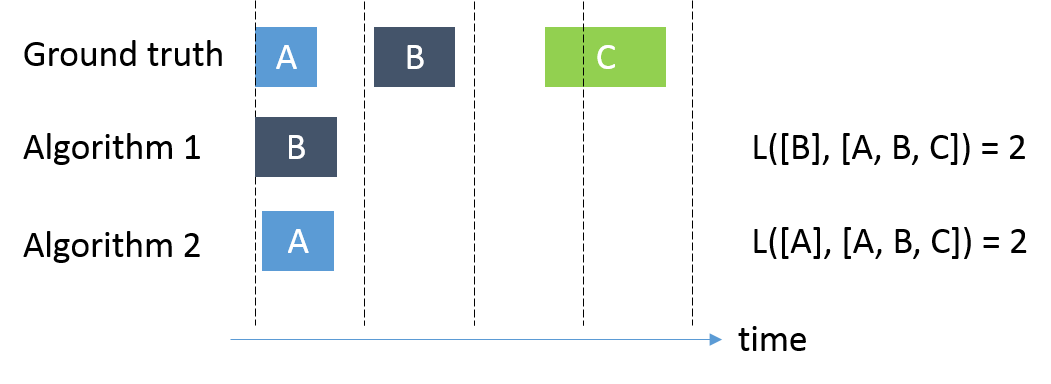
\includegraphics[width=0.8\textwidth]{figures/edit_distance.png}
\caption{Considering events as an ordered list without timing information does
not give a fair comparison for recognition performance. Applying the edit
distance score used in the challenges, both algorithms have 2 mistakes. However if
we consider the timing of the recognition, Algorithm 1 would have 3 mistakes.}
\label{fig:edit-distance}
\end{figure}

Song et al.~\cite{song12} and Morency et al.~\cite{morency07} used frame-based
metrics to evaluate their continuous gesture recognition systems. Frame-based
metrics consider timing inherently, but there are
artifacts, such as fragmenting and merge errors~\cite{ward11} in the results
that cannot be captured by this type of metrics. For example, in
Figure~\ref{fig:fragment}, Algorithm 1 has a higher frame-based TPR. However,
depending on the application, Algorithm 2 can have a better performance. Suppose we cast this example into a concrete scenario of a gesture-controlled presentation application, 
if the user does a ``swipe left'' gesture, using Algorithm 1, the system would
respond three times and change the slides three times; while using Algorithm 2,
the system would respond one time which is the desired outcome. The same
argument can also be made for merge errors (see Figure~\ref{fig:merge}). This
scenario shows that frame-based evaluation is less relevant for gestures
requiring discrete responses.

\begin{figure}[tbh]
\centering
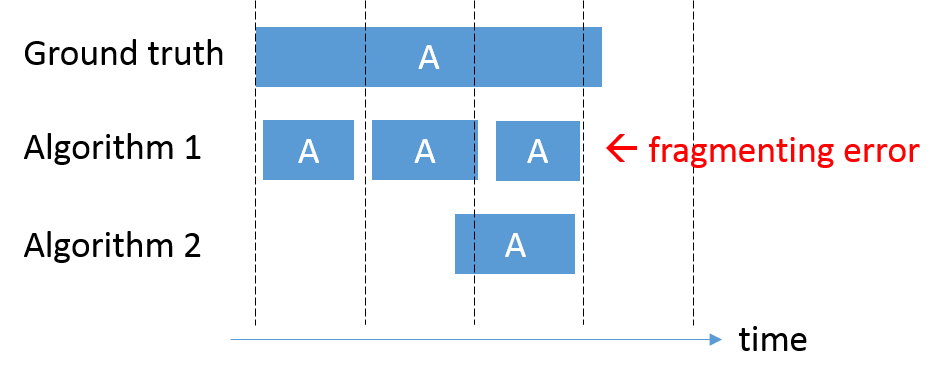
\includegraphics[width=0.8\textwidth]{figures/fragment.png}
\caption{Even though Algorithm 1 has a higher true positive rate, it has more
fragmenting errors. For certain applications, Algorithm 2 would have a better
performance.}
\label{fig:fragment}
\end{figure}

\begin{figure}[tbh]
\centering
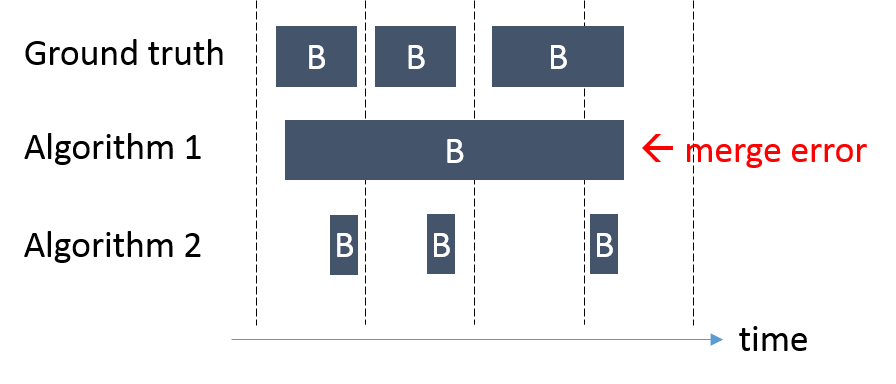
\includegraphics[width=0.8\textwidth]{figures/merge.png}
\caption{Even though Algorithm 1 has a higher true positive rate, it has more
merge errors. For certain applications, Algorithm 2 would have a better
performance.}
\label{fig:merge}
\end{figure}

There are situations where frame-based metrics are more relevant than
event-based metrics as well. Consider the same recognition results in
Figure~\ref{fig:fragment}, but this time gesture A is the ``point'' gesture
requiring continuous frame-by-frame response from the system (e.g., the system
shows a point cursor moving around according to where the user points at). In this case,
Algorithm 1, having a higher frame-based TPR, would have
better performance.

\section{Hybrid Performance Metrics}\label{sec:metrics} 
The examples in the previous section demonstrate the requirement of a hybrid
performance evaluation system. I believe that all three types of information -- frames, events and
timings -- are relevant for a real-time activity/gesture recognition system,
and should be included in the metric.
More importantly, as different categories of activities/gestures require
different kinds of responses from the system, it is necessary to identify
which metric is appropriate for which category of activities/gestures:  the event-based metric is
appropriate for discrete \textit{flow} gestures and the frame-based metric is
appropriate for continuous \textit{flow} gestures.

There are previous works that consider
hybrid metrics. Ruffieux et al.
combined a time-based metric with an event-based metric (see
Section~\ref{sec:chairgest-metric}). They included timing offset errors
explicitly in the metrics, but they did not consider frame-based metric. Ward et
al.~\cite{ward11} proposed a comprehensive scheme to combine both frame and
event scoring, but they did not consider how the different types of metrics are
relevant for different categories of activities.

The following section explains the details of the hybrid performance metric I
propose.

\subsection{Metric for Discrete Flow Gestures}
For discrete \textit{flow} (DF) gestures, the system responds at the end of the
nucleus phase, therefore the evaluation should be event-based. Let
$T_{{\text{gt\_start\_pre}}}$ be the ground truth start time of the pre-stroke phase and
$T_{{\text{gt\_stop\_post}}}$ be the ground truth stop time of the post-stroke
phase.
A recognized event is considered a TP if the time of response ($T_{\text{response}}$) 
occurs between $T_{{\text{gt\_start\_pre}}}$ and $T_{{\text{gt\_stop\_post}}} +
0.5\times(T_{{\text{gt\_stop\_post}}} -
T_{\text{gt\_start\_pre}})$.
We allow some margin for error because there can be small ground truth timing errors\footnote{Pre-stroke and post-stroke
timings are used because there may not be ground truth timings for nucleus
phases, such as in the YANG dataset. Manual labeling of the start and stop
timings of nucleus phases may be too time consuming.}.
Once a TP event is detected, the corresponding ground truth event is not
considered for further matching, so that multiple responses for the same gesture
(fragmenting errors) will be penalized. We then can compute event-based
precision, recall and $F_1$ score for DF gestures:
\begin{align}
\text{precision}^{\text{DF}} &=\frac{\text{\# TP DF events}}{\text{\# recognized
DF events}}
\\
\text{recall}^{\text{DF}} &=\frac{\text{\# TP DF events}}{\text{\# ground truth
DF events}} \\
F_1^{\text{DF}} &= 2\cdot \frac{\text{precision}^{\text{DF}} \cdot
\text{recall}^{\text{DF}}}{\text{precision}^{\text{DF}} +
\text{recall}^{\text{DF}}}
\end{align}

For discrete \textit{flow} gestures, we also define a Responsiveness Score (RS)
as the time difference in seconds between the moment when the system responds and the moment when the hand goes to a rest
position or changes gesture. Let $N_{TP}$ be the number of true positives, then
\begin{align}
RS = \frac{\sum_{i = 1}^{N_{TP}}T_{{\text{gt\_stop\_post}}} -
T_{\text{response}}}{N_{TP}}
\end{align}
A positive score means the responses are before the end of the post-strokes,
hence higher scores are better.

\subsection{Metric for Continuous Flow Gestures}
For continuous \textit{flow} (CF) gestures, the system responds frame by frame,
so it is more appropriate to use frame-based evaluation. For all the frames that are
recognized as continuous gestures, we can compute the number of TPs by
comparing them with the corresponding frames in the ground truth. Then, we can
compute frame-based precision, recall and $F_1$ score for all the frames
corresponding to CF gestures:
\begin{align}
\text{precision}^{\text{CF}} &=\frac{\text{\# TP CF frames}}{\text{\# recognized
CF frames}}
\\
\text{recall}^{\text{CF}} &=\frac{\text{\# TP CF frames}}{\text{\# ground truth
CF frames}}\\
F_1^{\text{CF}} &= 2\cdot \frac{\text{precision}^{\text{CF}} \cdot
\text{recall}^{\text{CF}}}{\text{precision}^{\text{CF}} +
\text{recall}^{\text{CF}}}
\end{align}


The average of the two $F_1$ scores can give an overall indication of the
performance of the system.
